\documentclass[sigconf, review=true, anonymous=true]{acmart}

\usepackage{booktabs} % For formal tables
\usepackage{algorithm}
\usepackage{algorithmic}
\DeclareMathOperator*{\argmax}{argmax}
\DeclareMathOperator*{\argmin}{argmin}

% Copyright
%\setcopyright{none}
%\setcopyright{acmcopyright}
%\setcopyright{acmlicensed}
%\setcopyright{rightsretained}
%\setcopyright{usgov}
%\setcopyright{usgovmixed}
%\setcopyright{cagov}
%\setcopyright{cagovmixed}


% DOI
%\acmDOI{10.475/123_4}

% ISBN
%\acmISBN{123-4567-24-567/08/06}

%Conference
%\acmConference[ICMR'17]{ACM Woodstock conference}{July 1997}{El Paso, Texas USA} 
%\acmYear{1997}
%\copyrightyear{2016}

%\acmPrice{15.00}


\begin{document}
\title{A Joint Model for Saliency Estimation and Video Localization}

\author{Haoyue Shi}
\affiliation{
  \institution{School of Electronics Engineering and Computer Science, Peking University}
  \city{Beijing, China} 
  \postcode{100871}
}
\email{hyshi@pku.edu.cn}

\author{Jia Chen}
\affiliation{
  \institution{Language Technologies Institute, Carnegie Mellon University}
  \city{Pittsburgh, PA, USA} 
  \postcode{15213}
}
\email{jiac@cs.cmu.edu.cn}

\author{Alexander G. Hauptmann}
\affiliation{
  \institution{Language Technologies Institute, Carnegie Mellon University}
  \city{Pittsburgh, PA, USA} 
  \postcode{15213}
}
\email{alex@cs.cmu.edu.cn}

% The default list of authors is too long for headers}

\begin{abstract}
\par
In this paper, we aim to determine the location of videos by matching the frames to a reference database, which contains plenty of geo-tagged images. We have demonstrated that salient regions (e.g. buildings) of a video frame (i.e. image) contains more information than non-salient regions (e.g. sky, roads and trees), so that the saliency score can perform as a guide in the matching procedure. In consideration of this fact, we propose a joint model based on a deep CNN architecture for both estimating saliency score and optimizing the matching between images guided by the saliency score in the training procedure. The experiments on Boston dataset and Tokyo 24/7 dataset have shown that our saliency aware method can help improve the accuracy of matching, and provide a reasonable explanation for the matched pairs. 
\end{abstract}

% \ccsdesc[300]{Specialized information retrieval~Image search} \\

% We no longer use \terms command
%\terms{Theory}

\keywords{Image Localization, Video Localization, Deep Learning}

\maketitle

\section{Introduction}
\par
Image geo-localization is a task which requires to use computer vision techniques to estimate the location (often GPS) of a given ground-level image by matching it to a reference database. In their previous work, Hays and Efros~\cite{hays2008im2gps} have proved the feasibility of this task by leveraging over 6 million GPS-tagged images from the Internet.
\par
There are already a lot of works focusing on the matching or image geo-localization task. Universal Correspondence Network\cite{choy_nips16} is an efficient method to extract features from images and solve such image localization problems by matching, while requiring patch-level labelled instances for training. Researchers have already released a lot of image-level labelled datasets. However, to the best of our knowledge, there isn't any large-scale patch-level labelled dataset for the task of image localization. What's more, NetVLAD~\cite{Arandjelovic16} proposed by Arandjelovic et al. is a nearly perfect method to solve the place recognition problem, which is very similar to image localization problem. But we still wonder whether we could align the matching score to patch-level. In other words, we aim to let the computer output the reason of why two images match or mismatch in patch-level, in order to further improve the performance for the image matching problem. In addition, real world may change everyday, especially when some event happens. To avoid the noise caused by daily events, we need some improvement on previous image localization/matching methods.
\par
Thus, we propose a method to solve the problem of cross-domain (event domain and satellite image database domain) video geo-localization by matching with weakly labelled (image level labelled rather than patch-level labelled) data, while the matching procedure is guided by the saliency of patches. In our method, the saliency of patches are estimated automatically without any further manual work.
\par
It's much easier for human beings to determine the geo-location for photographs of famous scenes rather than those of oceans, grasslands or even ordinary houses. This is because the famous scenes are rare, so that they are more discernible than oceans, grasslands and ordinary houses.
\par 
Similarly, buildings, especially famous buildings, are always more discernible than roads, trees, etc.  Figure~\ref{fig:library} is a photograph of Boston Public Library, McKim Building. When determining the geo-location of the image, we would focus on the discernible (salient) regions but not the non-salient ones, since only the former could provide us information about the location. In Figure~\ref{fig:library}, regions in red frames are salient while those in blue frames are not.
\begin{figure}[htbp]
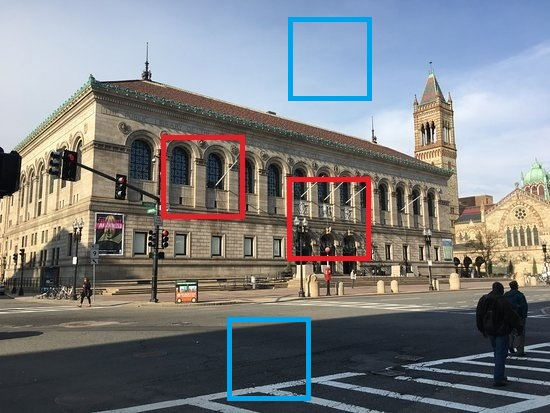
\includegraphics[width=0.41\textwidth]{img/library}
\\[0.1cm]
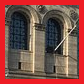
\includegraphics[width=0.1\textwidth]{img/library_1}
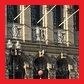
\includegraphics[width=0.1\textwidth]{img/library_2}
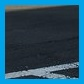
\includegraphics[width=0.1\textwidth]{img/library_3}

\includegraphics[width=0.1\textwidth]{img/library_4}
\caption{An example of salient regions and non-salient regions of an image.}
\label{fig:library}
\end{figure}
\par
Therefore, we aim to use the attribute of saliency to guide image/video localization. To estimate how salient a region is, we reconsider the fact that non-salient regions are less discernible. In other words, non-salient regions would be more common than salient ones in the database. We introduce the concept \textbf{saliency score} to measure how salient a region is. An intuitive idea is to set saliency score of a region inversely proportional to the number of its similar regions in the database. To evaluate how similar two regions are, we need to apply convolutional neural network (CNN), which has been widely used in the field of deep learning, to extract features from images. 
\par
In another hand, after estimating the saliency score of each region in an image. We propose an attention-based model to guide the geo-localization system to pay more attention to salient regions when localizing an image. Consequently, the model tends to be a joint model to both estimate saliency score of regions utilizing a matching model and optimize the matching model with the saliency score. 
\par
We evaluate our method on two video/image geo-localization datasets. The experimental result on Boston dataset have shown that our method works well on event video frame geo-localization task. We also evaluated it on the Tokyo Time Machine dataset~\cite{Arandjelovic16} in order to support the efficiency of our method.
\par
The contribution of this paper is threefold. 
\begin{enumerate}
\item We demonstrate that saliency is an effective attribute to guide image/video localization. 
\item We propose a method which can joint estimate the saliency score of image regions and geo-localize an image or a video.
\item Our method is helpful for real world event related video geo-localization and it is efficient to solve cross-domain matching problems.
\end{enumerate}



\section{Background and Related Work}
\subsection{Deep Learning}
\par
Deep learning is a technique which has been applied in the field of artificial intelligence, especially computer vision. It extract features of materials(usually images or videos) by learning deep neural networks. A lot of previous approaches have successfully utilized deep learning on the task of object recognition~\cite{krizhevsky2012imagenet}, faces recognition~\cite{taigman2014deepface} and place recognition~\cite{zhou2014learning,lin2015learning,Arandjelovic16,workman2015wide,weyand2016planet}. 
\subsection{Image/Video Geo-Localization}
\par
As we have mentioned in Section 1, early work by Hays and Efros~\cite{hays2008im2gps} revealed the feasibility of the image localization task. Zamir and Roshan~\cite{zamir2010accurate} used SIFT descriptors for image localization by voting, and constructed a dataset based on Google Street-View to test the efficiency of the algorithm. Lin et al.~\cite{lin2013cross} proposed the first ground-to-overhead geo-localization method, of which the key idea is to learn the relationship between the ground-level images and their over-head appearances. After that, Lin et al.~\cite{lin2015learning} then published an approach by CNN to learn deep representations for ground-to-overhead geo-localization. Vo and Hays~\cite{vo2016localizing} then explored several deep CNN architectures for the cross-domain matching and improved the accuracy of image geo-localization. What's more, Bansal et al.~\cite{bansal2012ultra} proposed a method to capture the structure of self-similarity of patterns on facades for image geo-localization.
\par
Leung et al.~\cite{leung2008localization} designed a monocular vision based particle filter localization system for urban settings that uses aerial reference map. However, because of the great similarity between the task of image localization and video localization, researchers often treat them as the same task.
\par
Visual place recognition is a similar task of image geo-localization. Arandjelovic et al.~\cite{Arandjelovic16} developed NetVLAD, a CNN architecture of which the main component is the VLAD (``Vectors of Locally Aggregated Descriptors'') layer and got the state-of-the-art performance on two challenging place recognition datasets. 

\subsection{Self-Paced Learning}
\par
In machine learning, a sequence of gradually  added training samples~\cite{bengio2009curriculum} is called a curriculum. Inspired by the cognitive process of humans and animals, a straightforward way to generate such a sequence is to add samples based on their ``easiness" to learn. However, such ``easiness" is based on specific problem and hard to generalize. In order to solve this problem, Self-Paced Learning (SPL) was introduced by Kumar et al.~\cite{kumar2010self}, which embeds curriculum designing into model learning. In SPL, the curriculum is gradually generated by the model itself based on what it has learned, and it's also a general implementation for curriculum learning. Following that, several works have improved self-paced learning~\cite{jiang2014easy, tang2012shifting, jiang2014self, jiang2015self}. In this paper, we propose self-paced learning method to automatically estimate the saliency score for each region of a frame.
\par
In self-paced curriculum learning, a the self-paced function $f(\mathbf{v};\lambda)$ determines a learning scheme~\cite{jiang2015self}, where $\mathbf{v}\in [0,1]^n$ denotes a vector of weight variable for each training sample and $\lambda$ controls the learning pace. In a self-paced function, $||\mathbf{v}||_1$ increases with respect to $\lambda$. For a fixed function $f(\mathbf{v};\lambda)$, the sample selecting weight $\mathbf{v}$ can be computed by 
\begin{equation}
\mathbf{v} = \argmin_{\mathbf{v}\in [0,1]^n}\sum v_il_i + f(\mathbf{v};\lambda)
\label{samplesel}
\end{equation} 
where $l_i$ is the loss function for the $i^{th}$ sample.

\subsection{Attention-Based Model}
While attention-based models are widely used in recognition tasks, many recent works show that attention-based model can improve the performance of machine learning models~\cite{mnih2014recurrent, zheng2015neural}. The key idea of attention-based model is to add attention information to build a representation. This idea is intuitive. For example, when looking at an image, we human beings often recognize the objects on it and then receive the information from the background, rather than receiving information simultaneously from the foreground objects and background scenes. In our approach, we compute the attention to each region by its saliency. 



\section{Methodology}
\par
\subsection{Problem Formulation}
\par
In the image/video geo-localization task, we have 
\begin{itemize}
\item A database $D_{train}$ which consists of images with GPS tags.
\item A training dataset. In the training dataset, we have an image set $Q_{train}$. Besides, we have the label set
$$Label_{train} = \{(q^{(i)}, d^{(j)}, l^{(i, j)}) | q^{(i)}\in Q_{train}, d^{(j)}\in D_{train}\}$$
which denote whether the image $q^{(i)}$ comes from the same region as the image $d^{(j)}$: $l^{(i, j)} = 1$ is for true and otherwise false. 
\item A separate database $D_{test}$ to be the reference in the localization procedure.
\item A separate query image set $Q_{test}$ in which all images require geo-localization by matching to $D_{test}$. 
\end{itemize}
Specially, $D_{test}$ can be the same as $D_{train}$.
\par
The problem we need to solve is to localize a query image/frame to the given database by finding the most similar image. We will define the similarity and describe our method in this section.  \\
\subsection{Saliency Score Estimation}
\par
Assuming we already have a pre-trained model for place recognition to project an image to a representative vector space, and our main purpose is to refine the model for better accuracy on the image geo-localization task. For the convenience of expression, let us first introduce some notations in Table~\ref{table:notations}. 
\begin{table}[htbp]
\begin{center}
\begin{tabular}{|c|p{0.35\textwidth}|}
\hline
$q_i$ & region $i$ in the query image $q$\\[0.2cm]
$d_j$ & region $j$ in the database image $d$\\[0.2cm]
$s(q_i), s(d_j)$ & the saliency of the region $q_i, d_j$, i.e. buildingness in our
task, ranged within $[0,1]$ \\[0.2cm]
$m(q_i, d_j)$ & matching score between region $q_i$ and $d_j$, where the better they match, the lower $m(q_i,d_j)$, since it's calculated by the distance between representing vectors\\[0.2cm]
\hline
\end{tabular}
\end{center}
\caption{Notations used in this section.}
\label{table:notations}
\end{table}
\par
As we expressed in Section 1, the basic assumption of our work is that salient regions have stronger ability to indicate the geo-location of an image. A salient region in an image would match less number of regions than non-salient ones. Inspired by the definition of inverse document frequency (IDF) which can be used to measure how much information a term(word) provides, an intuitive idea is to calculate the saliency score following Eq~\eqref{eq-1}.
\begin{equation}
s(q_i) \propto \sum_{d_j \in d, d \in D} m(q_i, d_j)
\label{eq-1}
\end{equation}
where $D$ denotes the set of all database images. The rationality can be understood in the following way. We can divide all the images into several classes, e.g. street, sky, trees and buildings, etc. For a non-salient region which belongs to the class $k$, the matching scores (distances in the feature space) between itself and other images in the class $k$ would be all small; however, for a salient (building) region which belongs to the class $p$, only several images in class $p$ have small distance with it, and it also mismatches with a large number of other images in its class, because the facades of builings could be very diverse. 
\par
Analogously, we can also compute the saliency score of database image regions. In order to normalize the saliency score, we compute $s(q_i)$ by Eq~\eqref{eq-2}.
\begin{equation}
s(q_i) = \frac{\sum_{d_j \in d, d \in D} m(q_i, d_j)}{\max_{q_k \in Q}\sum_{d_j \in d, d \in D} m(q_k, d_j) + \epsilon}
\label{eq-2}
\end{equation}
where $Q$ denotes the set of all query images, $\epsilon$ is a small constant number that guarantee the denominator would be positive. Both the denominator and numerator would be non-negative since $m(q_i, d_j)$ is calculated by the distance of the two regions in the feature space. What's more, we can compute the saliency score for database regions in the same way. 
\subsection{Saliency Guided Match Model Fine-tuning}
\par
We denote the pre-trained model for place recognition as $M$. Inspired by the work of Lin et al.~\cite{lin2015learning}, we could refine it by constructing a Siamese Network and modify the loss function between two images as following:
\begin{equation}
\label{eq-3}
L(q,d,l) = \sum_{q_i\in q} \frac{|q_i|}{|q|} L_s(q_i, d_j, l)
\end{equation}
where $q$ is a query image, $d$ is an image in the database, $q_i, d_j$ are sub-images of them, $|q|$ is the size of the image $q$, $l\in \{0,1\}$ denotes the label whether the two images are at the same place, $s(q_i)$ and $s(d_j)$ are the saliency scores of $q_i$ and $d_j$, $d_j$ is selected by $d_j = \argmin_{{d'} \in d} ||f(q_i), f({d'})||_2 $, and $L_s(q_i, d_j, l)$ can be computed with Eq~\eqref{eq-4}.
\begin{equation}
\label{eq-4}
L_s(q_i, d_j, l)=s(q_i)s(d_j)\frac{1}{2}lD^2 + \frac{1}{2}(1-l)\max(0,margin-D^2)
\end{equation}
where $D = ||f(q_i) - f(d_j)||_2$ is the Euclidean Distance of the two sub-images in the feature space, $m$ is a hyper-parameter which aims to keep a distance between negative samples in the feature space. In particular, $s(q_i)$ is fixed as well as $s(d_j)$ in this step. 
\par
According to Eq~\eqref{eq-3} and Eq~\eqref{eq-4}, we can modify the fine-tuning procedure of the match model from {\sl image pair based training} to {\sl region pair based training}. 

\subsection{Joint Saliency Estimation and Matching Optimization}
\par
We utilize the saliency score to guide the matching optimization and apply the updated match model to estimate more precise saliency score for each region of images. In other words, we are trying to teach the computer how much attention it need to pay to each region of the image by the saliency score. This can be done by an iterative procedure introduced in Algorithm~\ref{alg:joint} with applying self-pace learning with linear scheme. The self-paced function we applied is
\begin{equation}
f(\mathbf{v};\lambda) = \lambda-||\mathbf{v}||_1 = -\lambda\sum_{i=1}^n v_i
\label{selfpacedfunc}
\end{equation}
where $\mathbf{v}\in [0,1]^n$ denotes the vector of weight variable for each training sample, $\lambda$ is a hyper-parameter to control the pace of the learning procedure. The loss function when selecting training examples is
\begin{equation}
S(q_i, d_j) = -s(q_i) s(d_j) 
\label{eq-5}
\end{equation}
which is the additive inverse of the partial derivative of the loss function in the matching procedure, intuitively defined by the additive inverse of the product of saliency score of the image regions in each sample. The structure of our model is shown in Figure~\ref{fig:network}. By self-paced learning, we can let the system to learn ``easy'' samples first and then use the stronger model to learn more difficult samples. 
\par
Different from Lin et al.~\cite{lin2015learning}, we apply only one CNN rather than two seprate CNNs since the images in database and query may come from the same perspective of view.
\par
\begin{algorithm}
\begin{algorithmic}[1]  
\STATE{\textbf{set} saliency $\leftarrow$ uniform distribution}
\STATE{\textbf{set} $M$ = initial model}
\FOR{iteration $\leftarrow$ 1 to MAX\_ITERATION}
	\STATE{Estimate saliency socre with Eq~\eqref{eq-2}}
	\STATE{Select ``easy'' samples by Eq~\eqref{samplesel}\eqref{selfpacedfunc}\eqref{eq-5}}
	\STATE{Optimize $M$ with Eq~\eqref{eq-3} and Eq~\eqref{eq-4}}
	\STATE{Increase $\lambda$}
\ENDFOR
\end{algorithmic}
\caption{Joint Saliency Estimation and Matching Optimization}
\label{alg:joint}
\end{algorithm}

\begin{figure}[htbp]
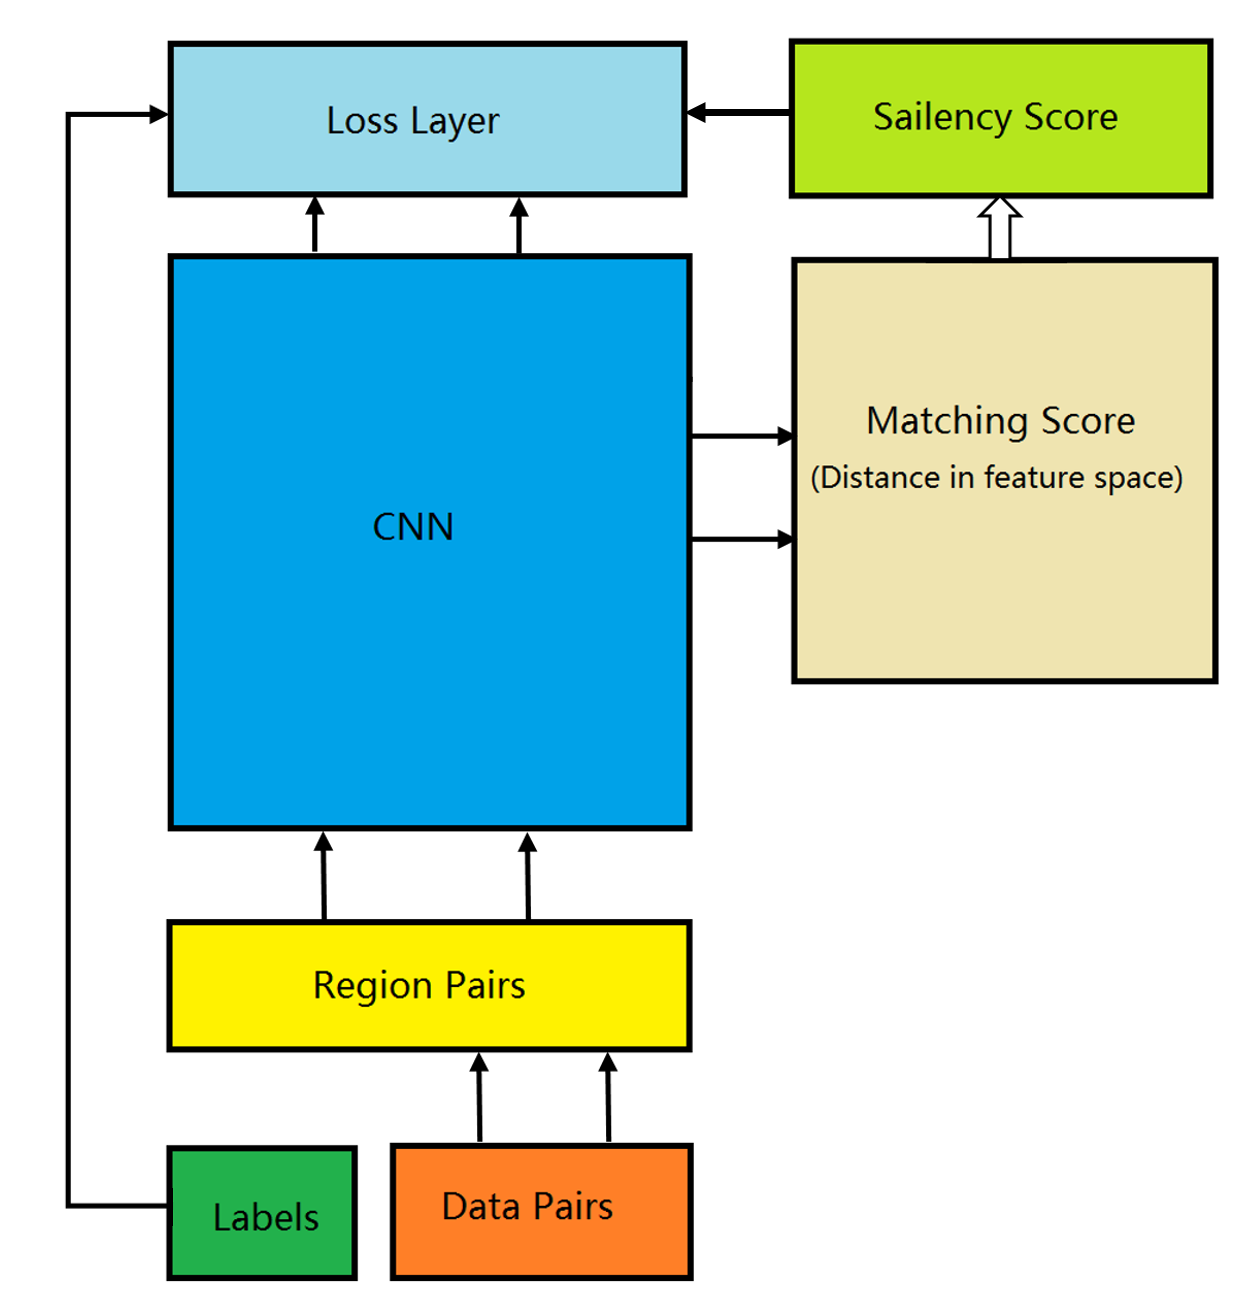
\includegraphics[width=0.9\linewidth]{img/structure}
\caption{The structure of our model.}
\label{fig:network}
\end{figure}

\subsection{Region-based Image/Video Frame Geo-Localization}
\par
When matching a query image/vdeo frame to the existing database, we propose two metrics to measure the similarity of two images. The first one is just the distance between two feature vectors of the images, which can be written as 
\begin{equation}
m(q, d) =  -||f(q) - f(d)||_2
\label{eq-6}
\end{equation}
where $f(q)$ and $f(d)$ are the vector representations of the two images in the feature space, computed by the match model $M$. The larger $m(q,d)$ is, the similar the images are. 
\par
For region-based image geo-localization, we divided an image into a ``pyramid'', where the first layer is the image itself, the second layer contains $2 \times 2$ sub-images and the third layer contains $3 \times 3$ sub-images. Thus, each image has 14 regions when we apply our saliency guided geo-localization method. The saliency score of each region is estimated separately. Figure~\ref{fig:pyramid} shows the dividing method visually. 
After dividing the images into regions, we could have a new metric to measure the similarity:
\begin{equation}
m_R(q,d) = -\sum_{q_i \in q} \min_{d_j\in d} \frac{|q_i|}{|q|} s(q_i)s(d_j) ||f(q_i)-f(d_j)||_2
\label{eq-7}
\end{equation}
 
\begin{figure}[htbp]
\includegraphics*[width=0.9\linewidth]{img/regions}
\caption{The regions of an image in our experiments.}
\label{fig:pyramid}
\end{figure}
\par
In the section of experiment, we will apply both the two metrics and compare them.

\section{Experiments}
\par
In the experiments, we use Caffe~\cite{jia2014caffe} as the deep learning framework and VGG-CNN-M~\cite{chatfield2014return} as the pre-trained model $M$ for match. 

\subsection{Datasets}
We applied our method on both Boston dataset and Tokyo Time Machine dataset. Before describing the experiments, let us first briefly introduce the two datasets. 

\subsubsection{Boston Dataset}
\par 
Chen et al.~\cite{chen2016boston} collected several video clips which are related to the event of Boston Marathon bombing from the internet. Our purpose is to geo-localize them to help the event re-construction. Figure~\ref{fig:bostonvideo} shows some samples of the video. Besides, we collected another 10,000 images around where the bombing happened from Google Map as the database. Figure~\ref{fig:dbregion} shows the region that our database covers. The colored masks are drawn by Google Map automatically, indicating the buildings. We sampled 2,500 GPS coordinate uniformly in such the region. For each GPS coordinate, we collected 4 image from 4 different perspectives of view. 
\begin{figure}[htbp]
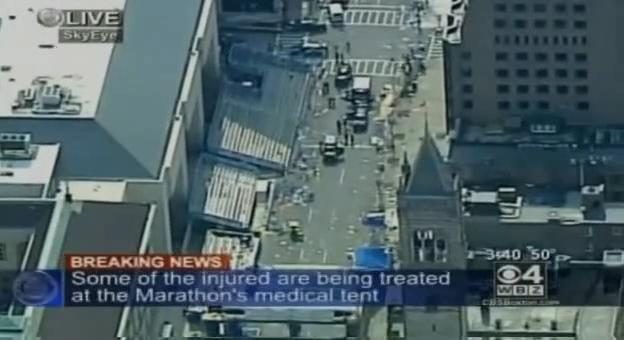
\includegraphics[width=0.45\linewidth]{img/video_1}
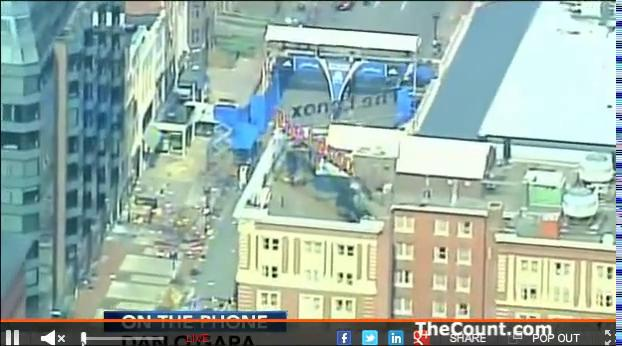
\includegraphics[width=0.45\linewidth]{img/video_2}
\\[0.1cm]
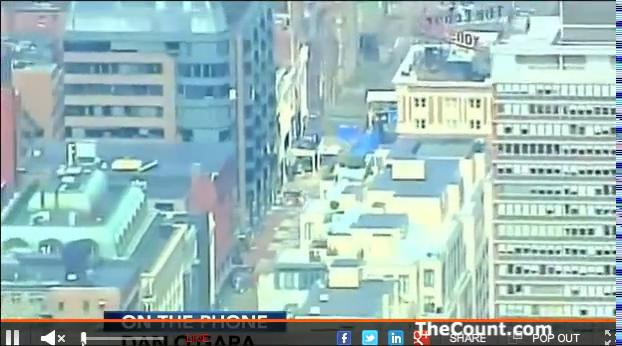
\includegraphics[width=0.45\linewidth]{img/video_3}
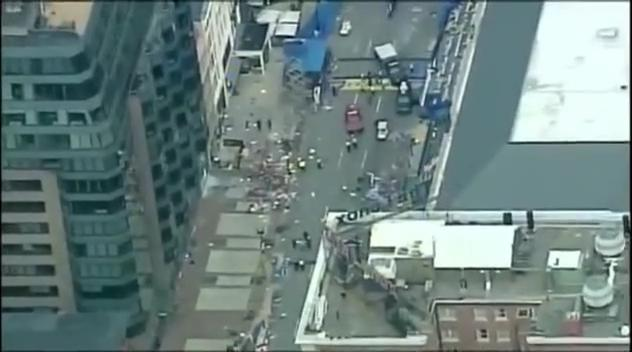
\includegraphics[width=0.45\linewidth]{img/video_4}
\caption{Sample video clips collected from the internet.}
\label{fig:bostonvideo}
\end{figure}
\begin{figure}[htbp]
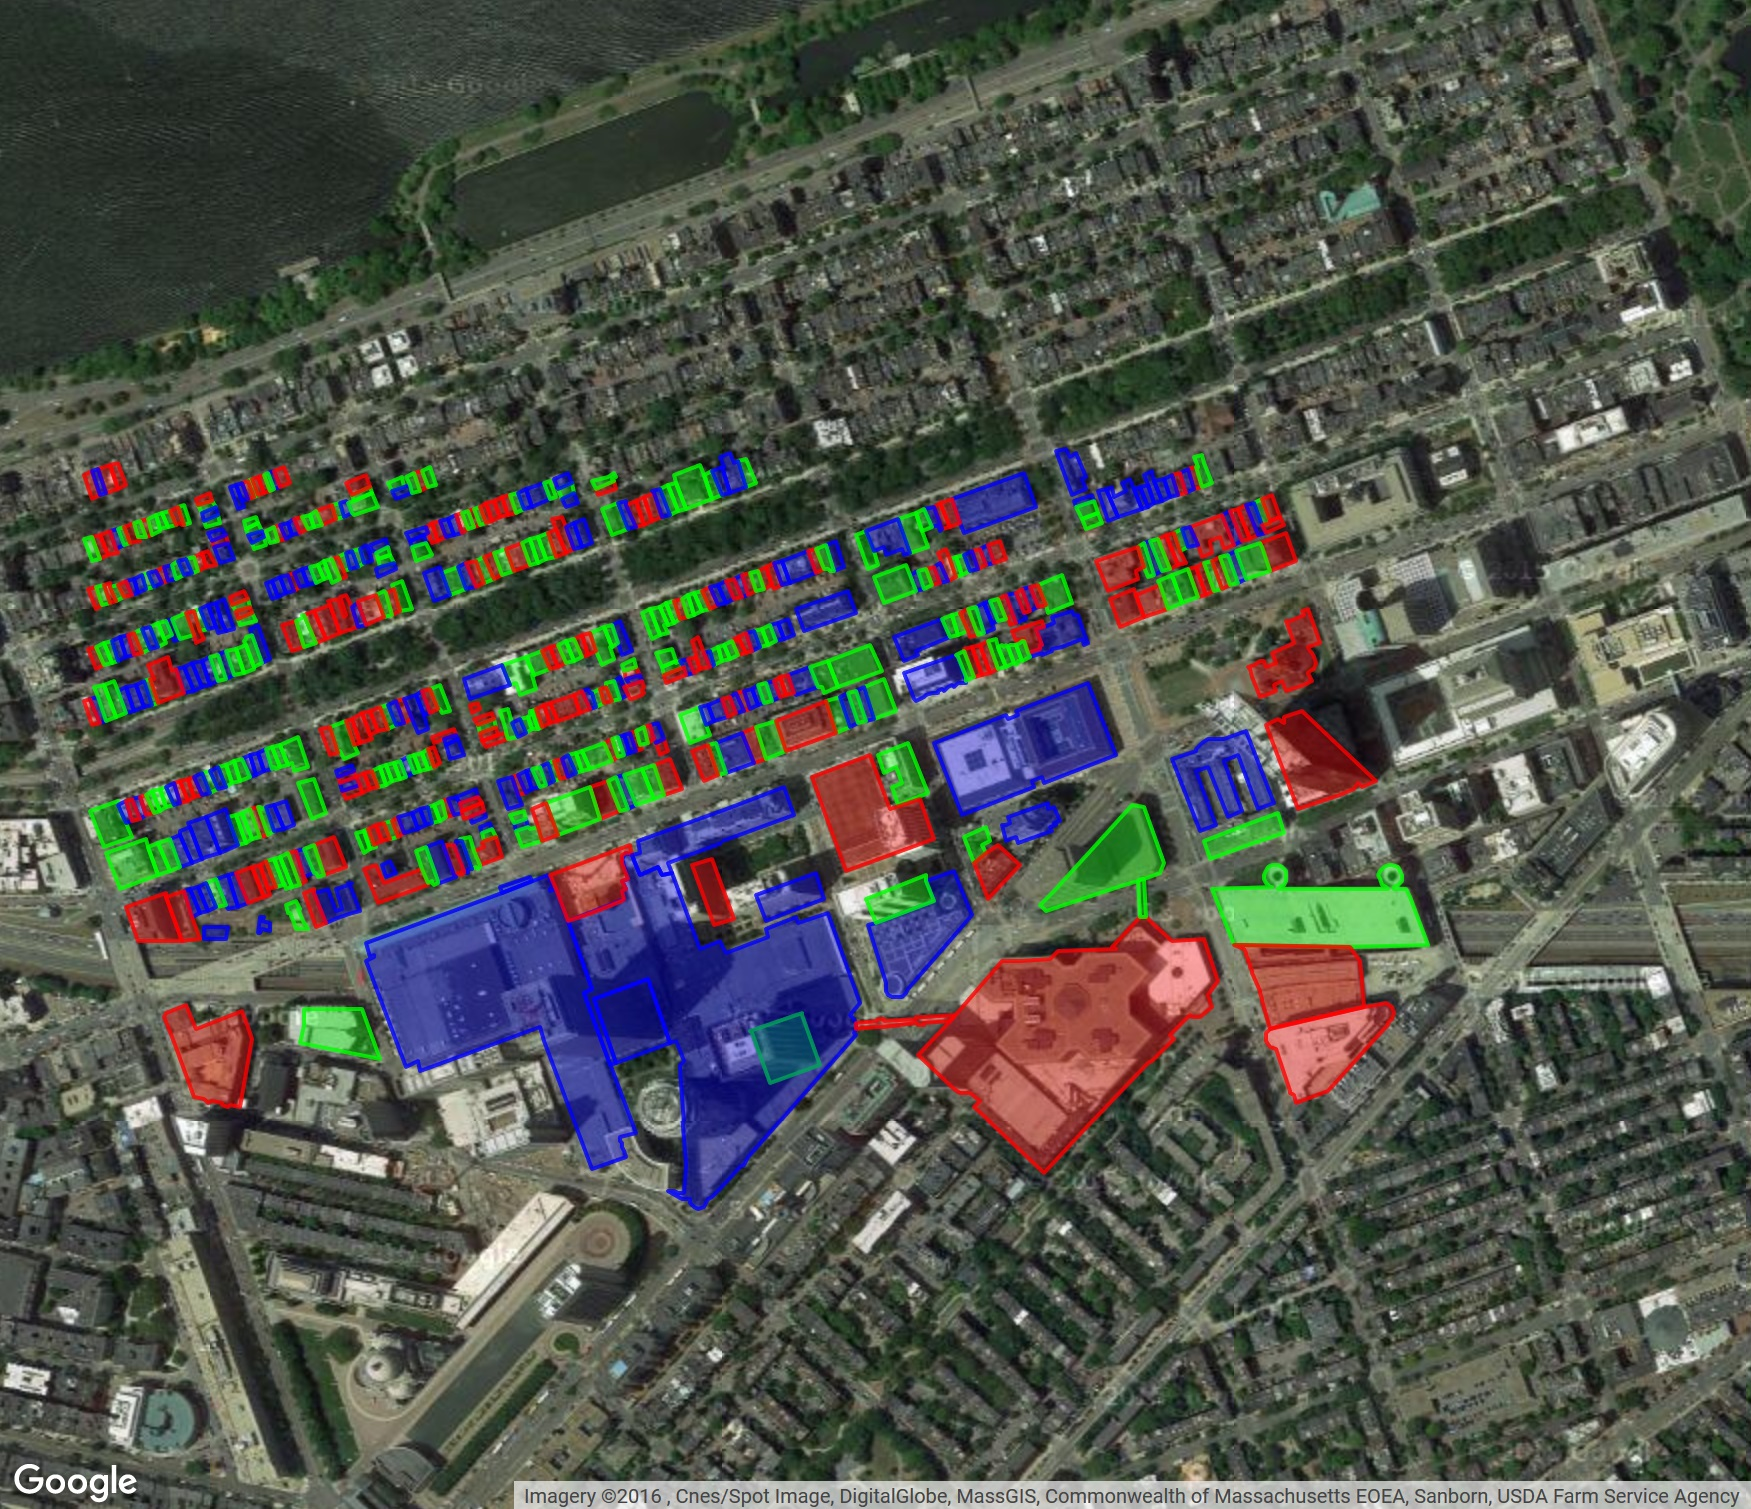
\includegraphics[width=0.92\linewidth]{img/db_region}
\caption{The region where the database of Boston dataset covers. }
\label{fig:dbregion}
\end{figure}

\subsubsection{Tokyo Time Machine Dataset}
\par

Tokyo Time Machine (TokyoTM) dataset was released by Arandjelovic et al.~\cite{Arandjelovic16}, generated  from  downloaded  Time  Machine  panoramas. 
\\
~\par
Table ~\ref{table:netvlad} shows  the  sizes  of  the two datasets we used. 

\begin{table}[htbp]
\begin{tabular}{l|rr}
Dataset & Database & Query set \\
\hline
\hline
Tokyo Time Machine-train & 49,104 & 7,277 \\
Tokyo Time Machine-val & 49,056 & 7,186 \\
Tokyo 24/7 (-test) & 75,984 & 1,125\\
\hline
Boston-train & 8,000 & 8,000 \\
Boston-val & 2,000 & 2,000 \\
Boston-test & 10,000 & 37 video clips
\end{tabular}
\caption{The size of the dataset we used in the experiments. The train/val(idation)/test dataset is mutually disjoint geographically. For the Boston train and validation dataset, we used data augmentation(zooming, rotating and translating) to transform images in database into query images. }
\label{table:netvlad}
\end{table}


\subsection{Optimizing Geo-Localization}
\par
We applied our method introduced in Section~3.4 and compared the result with VGG-CNN-M model as a baseline. In the following experiments, VGG-CNN-M-$m$ is the model released by Chatfield et al.~\cite{chatfield2014return}with the matching score $m$ computed by Eq~\eqref{eq-6}; VGG-CNN-M-$m_R$ is to estimate the saliency score using the VGG-CNN-M model, and then compute the match score between image $q$ and $d$ by Eq~\eqref{eq-7}; Ours-$m$ is to fine-tune the model by image-level pair matching (we report the result of it for comparison); Ours-$m_R$ is to optimize the model with Algorithm~\ref{alg:joint} and measure the similarity of images utilizing $m_R$. We also report the match result using the manually labelled saliency score for each region in query images, with the similarity measurement $m_R$, which should be the upper bound for such kind of matching models. 
\subsubsection{Experiments on Boston Dataset}
\par
We labelled the ground truth for 100 sample frames like those shown in Figure~\ref{fig:bostonvideo}, and computed mean average precision for the baseline model and our model. The result reported in Table~\ref{table:bostonresult} shows that our model has significantly improved the mean average precision (MAP) on the geo-localization task. For the convenience of view, Table~\ref{table:bostoncase} shows some case study on this task. In CNN, we resize the frames into $224 \times 224$ square shape. Thus, we show the frames and database in such a square shape rather than rectangular in Figure~\ref{fig:bostonvideo}.
\begin{table}[htbp]
\begin{tabular}{|l|l|}
\hline
Model & MAP ($\times 100$) \\
\hline \hline
VGG-CNN-M-$m$ & 28.85\\
VGG-CNN-M-$m_R$ & 35.67 \\
Ours-$m$ & 37.50 \\
Ours-$m_R$ & \textbf{58.33} \\
Manually-labelled-$m_R$ & 63.40 \\
\hline
\end{tabular}
\caption{The experimental result on Boston Dataset.}
\label{table:bostonresult}
\end{table}

\begin{table}[htbp]
\begin{tabular}{p{0.25\linewidth}|c|c|c|c}
Query Frame & 
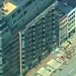
\includegraphics[width=0.15\linewidth]{img/case_1} &
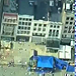
\includegraphics[width=0.15\linewidth]{img/case_2} &
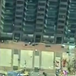
\includegraphics[width=0.15\linewidth]{img/case_3} &
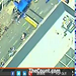
\includegraphics[width=0.15\linewidth]{img/case_4} \\
Ground Truth & 
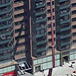
\includegraphics[width=0.15\linewidth]{img/case_1_grnd} &
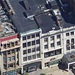
\includegraphics[width=0.15\linewidth]{img/case_2_grnd} &
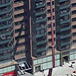
\includegraphics[width=0.15\linewidth]{img/case_3_grnd} &
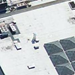
\includegraphics[width=0.15\linewidth]{img/case_4_grnd} \\
\hline
\multicolumn{5}{l}{\textbf{Ground Truth Ranking in All Database Images}} \\
\hline
VGG-CNN-M-$m$ & 6 & 3 & 10 & 108\\
Ours-$m_R$ & 1 & 1 & 1 & 12\\
\end{tabular}
\caption{Case study on Boston Dataset.}
\label{table:bostoncase}
\end{table}

\subsubsection{Experiments on TokyoTM Dataset}
\par
We compare our CNN representations trained for geo-localization againist the baseline. The representations all have 4096 dimensions, which is reduced automatically by fully connected layers in CNN. The result is shown in Table~\ref{table:netvlad-result}. 
\par
We then briefly discuss about the result. It proves the efficiency of our model, showing that our model obtains the best recall for every $N$. However, it's interesting that the model Ours-$m$ performs just around VGG-CNN-M-$m$, showing that saliency score is an important part in our model. It's not difficult to understand this fact, since the fine-tune procedure based only on the training dataset could easily cause over-fitting to the training data.

\begin{table*}[htbp]
\begin{tabular}{l|l|l|l|l|l|l|l|l|l}
\textbf{Model} & \textbf{N = 1} & \textbf{N = 2}& \textbf{N = 3}& \textbf{N = 4}& \textbf{N = 5}& \textbf{N = 10}& \textbf{N = 15} & \textbf{N = 20} & \textbf{N = 25} \\
\hline
VGG-CNN-M-$m$ & 0.0567&0.1017& 0.1442& 0.1797& 0.2033& 0.3286& 0.4657& 0.5816& 0.6832 \\

VGG-CNN-M-$m_R$ & 0.0591& 0.1087& 0.1584& 0.1868& 0.2104& 0.3617& 0.4728& 0.6147& 0.7092 \\

Ours-$m$ & 0.0757& 0.1158& 0.1560& 0.1891& 0.2317& 0.3404& 0.4657& 0.5579& 0.6809 \\

Ours-$m_R$ & 0.0922 & 0.1560 & 0.2128 & 0.2577& 0.2884&0.4870&0.6383&0.7423&0.8487 

\end{tabular}
\caption{The experimental result on TokyoTM test dataset (Tokyo 24/7). For each model, we report the recall when retrieving top $N$ images in database for each query ($N = 1, 2, 3, 4, 5, 10, 15, 20, 25$).}


\label{table:netvlad-result}
\end{table*}


\subsection{Saliency Estimation}
\par
In order to give a support to our method, we applied the following experiments to evaluate the saliency we estimated. 
\subsubsection{Qualitative Evaluation}
\par
To evaluate our method, we applied the method introduced in Section~3.1 to estimate the saliency score for each region of a given image. Figure~\ref{fig:saliency} shows the 8 most salient and 8 most non-salient regions in the Tokyo 24/7 database, while Table~\ref{table:saliencyscore}. We can easily see that the salient regions are all buildings with clear structure(1-8) while the non-salient regions are images from ``bad pictures''(9-11), trees(13-14), sky(15) and indiscernible building regions(12 and 16). 
\begin{figure}[htbp]
~\\[0.1cm]
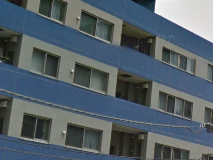
\includegraphics[width=0.2\linewidth]{img/sal_1}
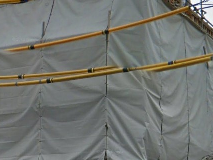
\includegraphics[width=0.2\linewidth]{img/sal_2}
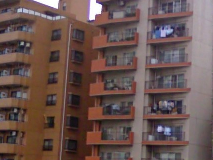
\includegraphics[width=0.2\linewidth]{img/sal_3}
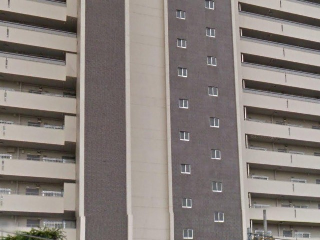
\includegraphics[width=0.2\linewidth]{img/sal_4}
\\[0.1cm]
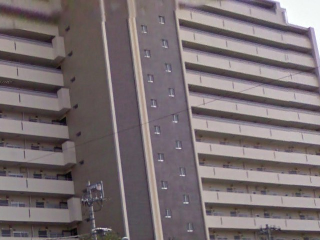
\includegraphics[width=0.2\linewidth]{img/sal_5} 
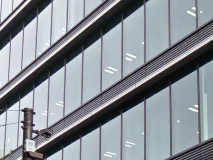
\includegraphics[width=0.2\linewidth]{img/sal_6} 
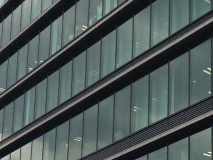
\includegraphics[width=0.2\linewidth]{img/sal_7} 
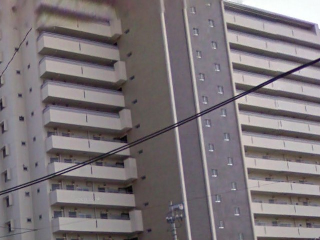
\includegraphics[width=0.2\linewidth]{img/sal_8} 
\\[0.3cm]

\includegraphics[width=0.2\linewidth]{img/nonsal_1}

\includegraphics[width=0.2\linewidth]{img/nonsal_2}

\includegraphics[width=0.2\linewidth]{img/nonsal_3}

\includegraphics[width=0.2\linewidth]{img/nonsal_4}
\\[0.1cm]
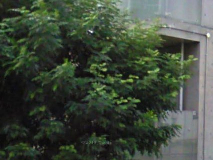
\includegraphics[width=0.2\linewidth]{img/nonsal_5}
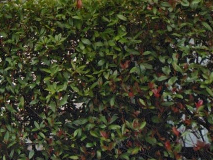
\includegraphics[width=0.2\linewidth]{img/nonsal_6}

\includegraphics[width=0.2\linewidth]{img/nonsal_7}

\includegraphics[width=0.2\linewidth]{img/nonsal_8}
\\
\caption{8 most salient regions(top) and 8 most non-salient regions in Tokyo 24/7 database.}
\label{fig:saliency}
\end{figure}

\begin{table}[htbp]
\begin{tabular}{r|r|r}
ID\# & Label & Saliency Score \\
\hline \hline
1 & salient & 1 \\
2 & salient & 0.982824053 \\
3 & salient & 0.980154725 \\
4 & salient & 0.974608251 \\
5 & salient & 0.960078978 \\
6 & salient & 0.950809385 \\
7 & salient & 0.929040028 \\
8 & salient & 0.928695266 \\
9 & non-salient & 0.322388817 \\
10 & non-salient & 0.324800642 \\
11 & non-salient & 0.325108224 \\
12 & non-salient & 0.327541606 \\
13 & non-salient & 0.328131344 \\
14 & non-salient & 0.328999699 \\
15 & non-salient & 0.329619018 \\
16 & non-salient & 0.330029754
\end{tabular}
\caption{Saliency socre of 8 most salient regions and 8 most non-salient regions.}
\label{table:saliencyscore}
\end{table}

\subsubsection{Quantitative  Evaluation}
\par
In order to show the efficiency of our saliency estimation method, we trained a separate model to estimate saliency score for each part. We manually labelled the saliency score for randomly selected 50 images (700 regions) in Tokyo 24/7 database. For each image, we use LabelMe~\cite{Russell2008} to label out the salient regions, and compute the saliency score of each region by the percentage of its salient part. 
\par
We report the Pearson correlation between the saliency score we computed with Eq~\eqref{eq-2} and that computed according to the manual labels. The Pearson correlation is $0.76259021$, showing that our estimated saliency score has strong relation with the ground truth saliency score. 


\section{Conclusion and Future Work}
\par
In this paper, we proposed a novel model that jointly estimates saliency score and optimizes geo-localization for street view or aerial images, by matching it to a geo-tagged database. When optmizing the matching model, we applied self-paced learning algorithm. The experimental results have shown that our method can help to improve the performance of image/video geo-localization on two challenging image/video geo-localization dataset, and proved the efficiency of self-paced learning algorithm.
\par
Besides, we have demonstrated that saliency is a very well guide on image geo-localization tasks, and it can be estimated just by image matching models with only the weakly labelled datasets, which doesn't need any further difficult manual work. This conclusion can shed light to the solutions to other matching or saliency estimating problems. 
\par
Due to the limitation of the computing time, the initial model for matching we applied in our experiments on the joint optimization is VGG-CNN-M. However, the state-of-the-art model on such kind of problem (NetVLAD) outperforms it significantly. In the future work, we should consider to apply the released NetVLAD model as the initial model in order to obtain a better result for image geo-localization.


\bibliographystyle{ACM-Reference-Format}
\bibliography{sigproc} 

\end{document}
